\documentclass[../../main.tex]{subfiles}

\begin{figure}[ht]
    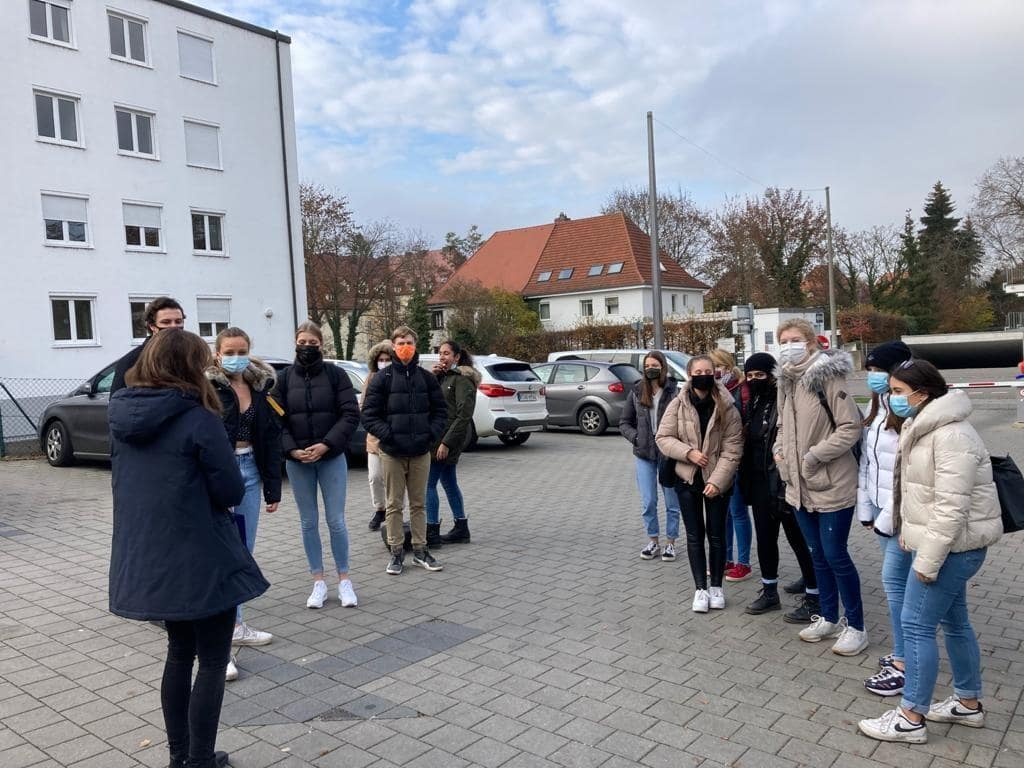
\includegraphics[width=\textwidth]{foto_hedwigsklinik_designvorstellung_2.jpg}
\end{figure}

Wir haben uns wieder mit den Leitern der Hedwigsklinik getroffen, um einen ersten Einblick in die Visualisierung der Hedwigsklinik zu erhalten. Eine 3D-Animation wurde vorgestellt, welche die neue Hedwigsklinik von außen, und auch Eingabgsbereich und Cafeteria zeigt.

Ich halte das Design auf derzeitigem Stand für beeindruckend, finde es aber teilweise zu Farbenfroh. Die Farben an der Außenwand sollten meiner Meinung nach minimal gehalten werden, weil es so moderner ist. Ich denke, die Cafeteria ist am besten gelungen. Das Glaskuppeldach und das schlichte Innendesign gefällt mir.